\begin{figure}
	\centering
	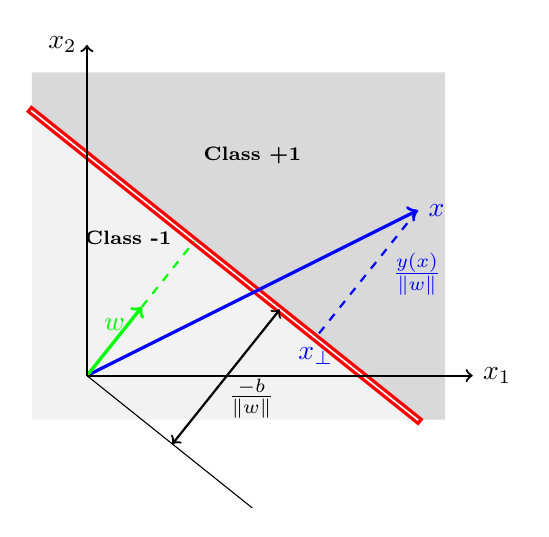
\begin{tikzpicture}[
		scale=0.7
	]

		\fill[fill=gray,fill opacity=0.3] (-1,4.8) -- (-1,5.5) -- (6.5,5.5) -- (6.5,-0.8) -- (6,-0.8) -- cycle;
		\fill[fill=lightgray,fill opacity=0.2] (-1,4.8) -- (-1,-0.8) -- (6,-0.8) -- cycle;

		\draw[very thick,double,line cap=rect,red] (-1,4.8) -- (6,-0.8);
		\draw[very thick,blue,->] (0,0) -- (6,3) node[right] {$\bm{x}$};
		\draw[thick,dashed,blue] (6,3) -- node[right=2mm] {$\frac{y(\bm{x})}{\Vert \bm{w} \Vert}$} (4.15,0.69)
			node[below] {$\bm{x}_{\perp}$};
		\draw[very thick,green,->] (0,0) -- node[above] {$\bm{w}$} (1,1.25);
		\draw[thick,dashed,green] (1,1.25) -- (1.95,2.44);
		
		\draw (0,0) -- (3,-2.4);
		\draw[<->,thick] (3.5,1.2) -- node[below right=-1mm] {$\frac{-b}{\Vert \bm{w} \Vert}$} (1.55,-1.24);

		% axes
		\draw[thick,->] (0,0) -- (7,0) node[right] {$x_1$};
		\draw[thick,->] (0,0) -- (0,6) node[left] {$x_2$};

		\node at (3,4) {\scriptsize\textbf{Class +1}};
		\node at (0.75,2.5) {\scriptsize\textbf{Class -1}};

	\end{tikzpicture}
\end{figure}